\documentclass{scrartcl}

\usepackage[utf8]{inputenc}


% zus�tzliche mathematische Symbole, AMS=American Mathematical Society 
\usepackage{amssymb}
\usepackage{amsmath}
\usepackage{amsthm}
\usepackage{bbm}
\usepackage{color}
\usepackage{listings}
\usepackage{pdfpages}
\usepackage{csquotes}
\usepackage{float}

% f�rs Einbinden von Graphiken
\usepackage{graphicx}

% f�r Namen etc. in Kopf- oder Fu�zeile
\usepackage{fancyhdr}
\usepackage{tikz}
\usetikzlibrary{arrows, automata}

% erlaubt benutzerdefinierte Kopfzeilen 
\pagestyle{fancy}

% Definition der Kopfzeile
\lhead{
\begin{tabular}{lll}
Maciej Janowski \\
\end{tabular}
}
\chead{}
\rhead{\today{}}
\lfoot{}
\cfoot{Seite \thepage}
\rfoot{} 

\begin{document}

\section*{LAB}
\subsection*{Task}
Main part of our assignemnt was to implement a behavioral cloning agent and evaluate its performance. We had to collect training data, create a model, then train it and test it in OpenAI Gym benchmark suite.

\subsection*{Architecture of the network}

\begin{table}[h]
	\centering
\begin{tabular}{|c||c|c||c||c|}
	\hline
	\textbf{Layer} & \textbf{Filter size} & \textbf{Number of filters} & \textbf{Activation function} & \textbf{Use pooling}  \\ \hline \hline
	Convolutional layer & 3 & 16 & ReLU & yes \\ \hline
	Convolutional layer & 3 & 32  & ReLU & yes \\ \hline
	Convolutional layer & 3  & 32 & ReLU & yes \\ \hline
	Convolutional layer & 3 & 32 & ReLU & yes \\ \hline
	Flatten layer & -  & - & - & -  \\ \hline
	Fully Connected layer  & - & - & ReLU & - \\ \hline
	Fully Connected layer  & - & - & - & - \\ \hline	
\end{tabular}
\caption{Parameters for each layer}
\end{table}

\subsection*{Performance}

\begin{figure}[H]
	\centering
	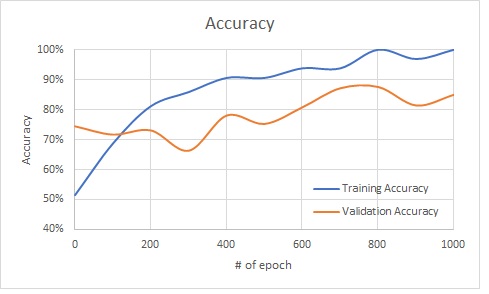
\includegraphics[scale=0.6]{Accuracy}
	\caption{Learning curve}
	\label{fig:1}
\end{figure}


\subsection*{Comments}

\begin{itemize}
	\item It was really important to make training data useful. Most of the data was teaching our model not to do anything. That is why, I had to implement some kind of method to deal with that problem. I decided to assign probability of adding each data sample to training set according to its distribution in player's actions. It solved problem, as in each mini batch was feeding the model with all actions. 

	\item Another approach I tested was to translate idle action to accelerating with some probability, to make the car go faster.
	\item Unfortunately after today's work test-agent script stopped working for me, so I cannot record scores for the agent.
	\item I will try to fix that problem as soon as possible and push changes to the repository.
\end{itemize}
\end{document}


